\documentclass[11pt,a4paper]{article}
\usepackage[backend=biber]{biblatex}
\usepackage{graphicx}
\usepackage{subcaption}
\usepackage{pgfplots}
\usepackage[top=1in, bottom=1.25in, left=0.5in, right=0.5in]{geometry}
\usepackage[hidelinks]{hyperref}

\addbibresource{references.bib}
\pgfplotsset{compat=1.15}

\begin{document}

\title{Fault Detection}
\author{Danil Kuzin \\ \texttt{danilkuzin@gmail.com}}
\date{January-March 2019}
\maketitle

\abstract
This report presents the results of the work done for geological faults detection with deep learning methods.



\section{Introduction}
Deep learning methods are usually used for the machine learning problems when features of the data are complex and it
is not possible to extract them manually. This includes speech recognition with different phonemes, text translation
with different meanings of words depending on the context, or image recognition with a large variety of shapes. Training
of deep learning models usually requires large datasets, but the trained models can produce results that are better than
of human experts for these problems.

We consider the deep learning approach for the problem of geological faults detection. Faults appear as a results of
land masses moving and can be dangerous to the people leaving nearby as they can cause earthquakes when they continue to
move. While in some regions, such as US these areas are well-researched, there are large regions remaining, such as Tibet,
or Iran, that lack the detailed maps of faults.

We are using only the satellite images of the earth surface, which allows to inexpensively process large amounts of areas
once the model was trained. The results of training on one of the region can be potentially transferred into other regions
without, or with little additional training.

We believe that deep learning approach can automatically recognise image features that are related to faults in a wide
variety of image bands and may even lead to reconsidering existing on-site approaches for fault detection, like the
deep-learning AlphaGo system has introduced new strategies in the game of Go even for the professional players.

The relevant literature includes: training CNNs on synthetic and real seismic data for faults
detection~\cite{pochet2018seismic, araya2017automated, xiong2018seismic, chehrazi2013seismic, lu2018using, hale2014}.
But most of these works include other data from the seismic images, or don't consider the real data. We are using the
professionally-mapped real data for training and performance evaluation.

%The other literature on detection from satellite images includes: detecting roads on pixel level from lots of satellite
%images and then denoising to get connected nets \cite{mnih2010learning},

\section{Data}

We obtained the satellite images from the Landsat-8 satellite and elevation data from the Opentopography: Shuttle Radar
Topography Mission (SRTM GL1) Global 30m.

The full list of channels is:
\begin{itemize}
\item \textit{Red, Green, Blue} - visible spectrum from Landsat-8
\item \textit{Elevation} - elevation data from SRTM
\item \textit{Slope} - estimated based on elevation with Geospatial Data Abstraction Library
\item \textit{Coastal} - ultrablue band, useful for coastal water and aerosol studies from Landsat-8
\item \textit{Near Infrared} - useful for biomass content and shorelines from Landsat-8
\item \textit{Short-wave Infrared 1} - useful for moisture content of soil and vegetation from Landsat-8
\item \textit{Short-wave Infrared 2} - useful for moisture content from Landsat-8
\item \textit{Panchromatic} - finer resolution from Landsat-8
\item \textit{Erosion} - the estimted difference from the smoothed image
\item \textit{Curvature} - the estimated Hessian of the elevation
\item \textit{Thermal Infrared 1} - thermal mapping and estimated soil moisture from Landsat-8
\item \textit{Thermal Infrared 2} - thermal mapping and estimated soil moisture from Landsat-8
\end{itemize}

For neural networks data is usually normalised, so that the input data comes from the same distribution. Given that we
have different regions, several potential options for normalisation were possible: normalise with mean and variance
estimated for all images, or for every image independently. In the former case we better estimate the parameters, but
the latter case allows to sequentially process more data, without reestimating statistics for the previous images. In
our approach we normalised RGB images with an assumption of uniform distribution in [0, 255] interval
(the Landsat data was converted to that interval first). For other channels we independently estimated mean and variance.

The fault lines and fault lookalikes were labelled on some of the regions. Fault lookalikes are the lines and areas that
contain the features similar to the real faults but are not faults. Adding this class helps in choosing the right data
to train and estimating the quality of the training.

The examples of labelled data and channels are shown in the \figurename~\ref{fig:features}.

The whole datasets include:
\begin{enumerate}
\item Lopukangri (Tibet) of size $100 km \times 100 km$ --- internal labels of the part of the area
\item Muga Puruo (Tibet) of size $100 km \times 100 km$ --- internal labels of the part of the area
\item Muggarboibo (Tibet) of size $100 km \times 100 km$ --- no labels, test data
\item Austin-Tonopah (US) of size $100 km \times 100 km$ --- no labels, test data
\item Las Vegas Nevada (US) of size $100 km \times 100 km$ --- no labels, test data
\item Izmir (Turkey) of size $100 km \times 100 km$ --- no labels, test data
\item Nevada Training (US) of size $200 km \times 400 km$ --- public labels of the part of the whole area
\item Nevada Test (US) of size $200 km \times 400 km$ --- public labels of the part of the whole area
\end{enumerate}

\begin{figure}[t]
    \centering
    \begin{subfigure}[b]{0.18\textwidth}
        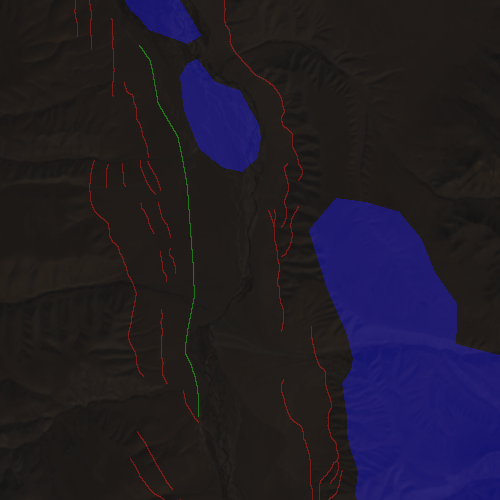
\includegraphics[width=\textwidth]{graphics/data/0/features_optical_rgb.png}
        \caption{Optical RGB}
        \label{fig:features_optical_rgb}
    \end{subfigure}
    ~
    \begin{subfigure}[b]{0.18\textwidth}
        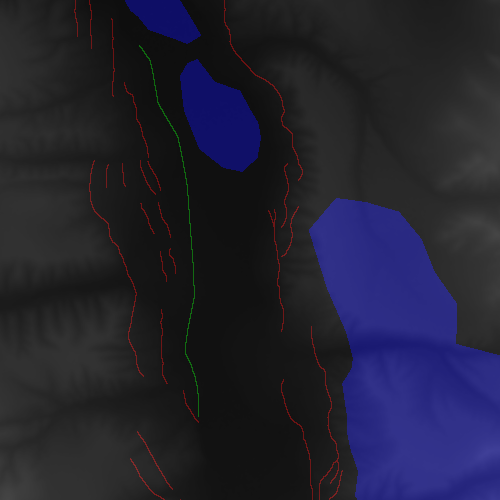
\includegraphics[width=\textwidth]{graphics/data/0/features_elevation.png}
        \caption{Elevation}
        \label{fig:features_elevation}
    \end{subfigure}
    ~
    \begin{subfigure}[b]{0.18\textwidth}
        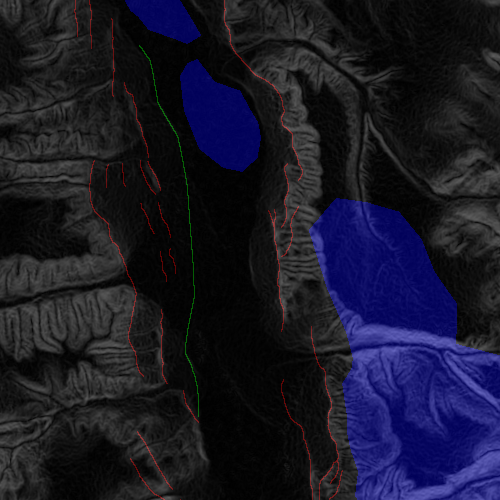
\includegraphics[width=\textwidth]{graphics/data/0/features_slope.png}
        \caption{Slope}
        \label{fig:features_slope}
    \end{subfigure}
    ~
    \begin{subfigure}[b]{0.18\textwidth}
        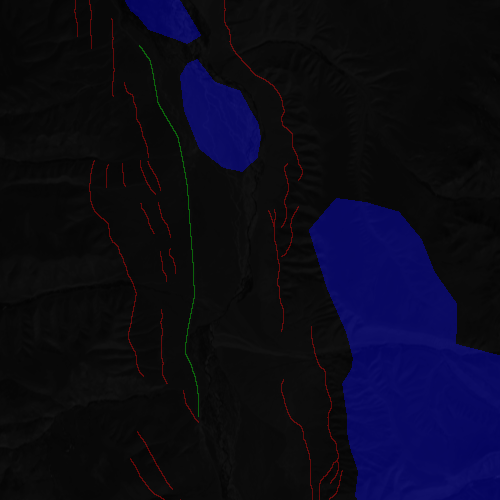
\includegraphics[width=\textwidth]{graphics/data/0/features_ultrablue.png}
        \caption{Coastal}
        \label{fig:features_ultrablue}
    \end{subfigure}
    ~
    \begin{subfigure}[b]{0.18\textwidth}
        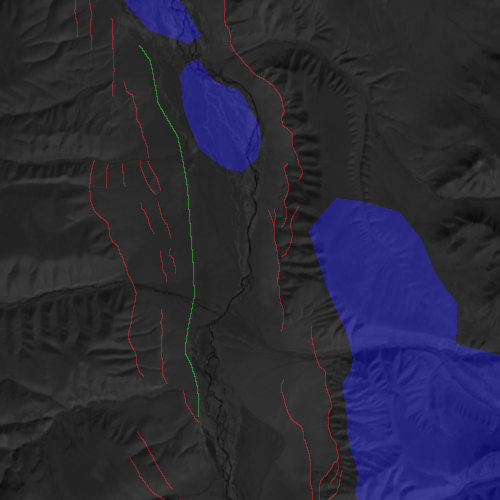
\includegraphics[width=\textwidth]{graphics/data/0/features_nir.png}
        \caption{NIR}
        \label{fig:features_nir}
    \end{subfigure}

    \begin{subfigure}[b]{0.18\textwidth}
        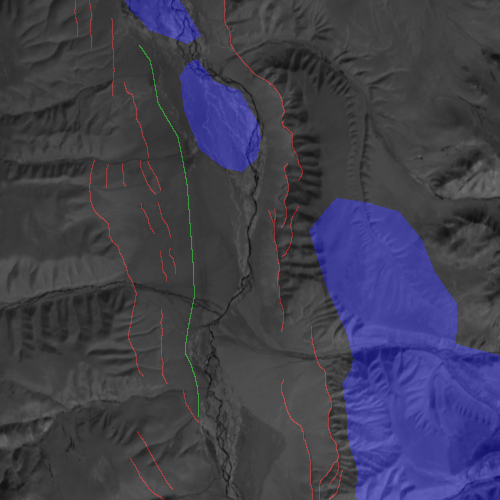
\includegraphics[width=\textwidth]{graphics/data/0/features_swir1.png}
        \caption{SWIR1}
        \label{fig:features_swir1}
    \end{subfigure}
    ~
    \begin{subfigure}[b]{0.18\textwidth}
        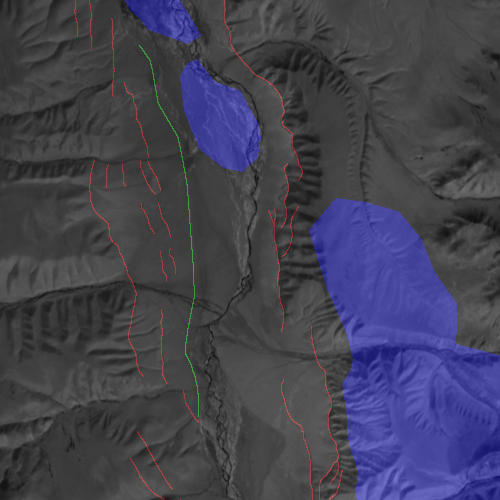
\includegraphics[width=\textwidth]{graphics/data/0/features_swir2.png}
        \caption{SWIR2}
        \label{fig:features_swir2}
    \end{subfigure}
    ~
    \begin{subfigure}[b]{0.18\textwidth}
        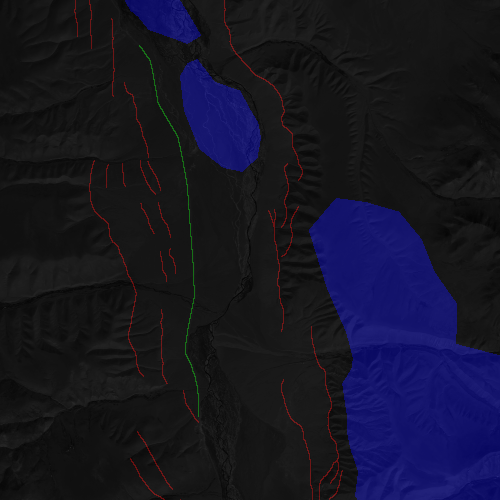
\includegraphics[width=\textwidth]{graphics/data/0/features_panchromatic.png}
        \caption{Panchromatic}
        \label{fig:features_panchromatic}
    \end{subfigure}
    ~
    \begin{subfigure}[b]{0.18\textwidth}
        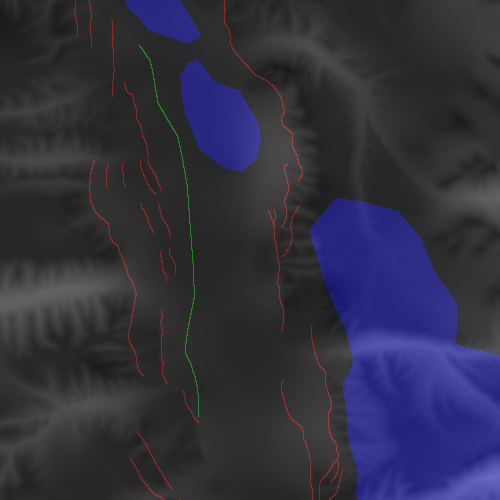
\includegraphics[width=\textwidth]{graphics/data/0/features_erosion.png}
        \caption{Erosion}
        \label{fig:features_erosion}
    \end{subfigure}
    ~
    \begin{subfigure}[b]{0.18\textwidth}
        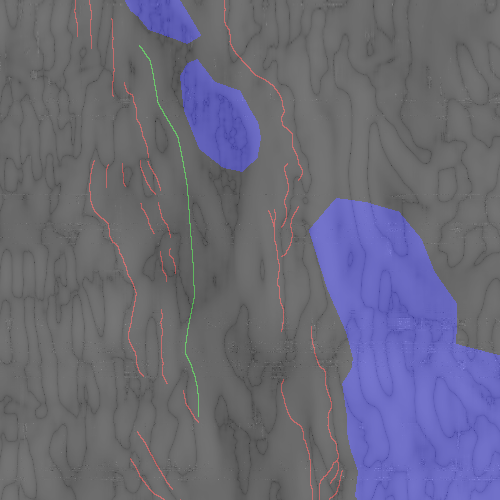
\includegraphics[width=\textwidth]{graphics/data/0/features_curve.png}
        \caption{Curvature}
        \label{fig:features_curve}
    \end{subfigure}
    \caption{Labelled features for a subset of Tibet data}\label{fig:features}
\end{figure}

\section{Neural network}
Neural networks consist of a set of layers that transform the input data into the output prediction via simple
transformation functions and nonlinear functions. A lot of architectures have been developed recently, such as recurrent
layers to model sequential features, autoencoders to find the most relevant features, or attention mechanisms to focus
on most relevant areas.

We base the architecture on the LeNet-5 net~\cite{lecun1998gradient}, that was originally used for handwritten digits
recognition as usually used for benchmarking nowadays. It contains two levels of convolutions that usually can learn to
detect simple relationships for nearby pixels. The more complex architectures, such as AlexNet, ResNet, VGGNet, Inception
contain much deeper convolutions that can learn to recognise more difficult structural patters, but they require longer
training on larger amount of data. Experiments with higher (up to 5 convolutional) number of layers demonstrated that
the current amount of training data is not enough to utilise the advantages of more complex architectures.

Our architecture is described below. The meaning of each layer can be found in the deep learning literature, such
as~\cite{cnn-tutorial}.

\begin{enumerate}
\item \textit{Input Layer} of shape \textit{patch width} $\times$ \textit{patch height} $\times$ \textit{number of features}
\item \textit{2D convolution} with $32$ filters of $5 \times 5$ kernel size
\item \textit{Relu} activation
\item \textit{MaxPooling2D} with $2 \times 2$ pool size
\item \textit{2D convolution} with 64 filters of $5 \times 5$ kernel size
\item \textit{Relu} activation
\item \textit{MaxPooling2D} with $2 \times 2$ pool size
\item \textit{Flatten} layer
\item \textit{Dense} with $1024$ units
\item \textit{Relu} activation
\item \textit{Dropout} with $0.5$ rate
\item \textit{Dense} layer with $2$ units corresponding to output classes
\item \textit{Softmax} activation
\end{enumerate}
Categorical crossentropy function is used for loss estimation, it estimates how well predicted labels match given labels.
Then the gradient of the loss is used to update the layer weights.


\section{Experiments}
To visualise the predictions we create the heatmaps for fault probabilities at each region. The sequential patches
taken with stride of 10 pixels from the original images are fed into the neural network, and the fault probabilities are
recorded for all pixels within that area. Then the fault probabilities are averaged for all pixels as an exp of the
average log.


\subsection{Train on Tibet data}
For this experiment we sample 2000 patches of size 150x150 pixels (5km x 5km) from each of the Tibet regions 1 and 2,
randomly rotated and flipped, with probabilities 0.5 from faults, 0.25 from lookalikes, 0.25 from nonfaults, so we have
approximately 2000 fault patches and 2000 non-fault patches, 80% of which are used for training, 20% for validation.

Faults and fault lookalikes are marked with lines, we sample random points from these lines and create patches with
centers at these points. Non-fault areas are marked with polygons, we sample patches that fully lie within the marked
polygon. We fix this dataset in advance and train a neural net on it after that.

We run the training for 30 epochs. At every epoch the whole sampled dataset is divided into minibatches of size 32 and
they are iteratively fed into the neural network, and the gradient of the classification loss is backpropagated through
it to update the weights of the neural network.

\figurename~\ref{train_on_01_features_01234_no_additional} presents the performance during training. As after 10th
iteration the validation score does not considerably improve, we use the weights obtained at this iteration for predictions.

\begin{figure}[t]
\centering
    \begin{subfigure}[b]{0.45\textwidth}
        \scalebox{0.9}{
            \begin{tikzpicture}
            \begin{axis}[axis lines=left, xlabel=epoch, legend style={at={(0.97,0.6)},anchor=east}]
            \addplot[solid, color=orange] table[x=epoch, y=val_acc, col sep=comma]
            {graphics/training/train_on_01_features_01234/log.csv};
            \addlegendentry{val acc}
            \addplot[dashed, color=orange] table[x=epoch, y=acc, col sep=comma]
            {graphics/training/train_on_01_features_01234/log.csv};
            \addlegendentry{acc}
            \addplot[solid, color=cyan] table [x=epoch, y=val_loss, col sep=comma]
            {graphics/training/train_on_01_features_01234/log.csv};
            \addlegendentry{val loss}
            \addplot[dashed, color=cyan] table [x=epoch, y=loss, col sep=comma]
            {graphics/training/train_on_01_features_01234/log.csv};
            \addlegendentry{loss}
            \end{axis}
            \end{tikzpicture}
        }
        \caption{Training on Tibet data}
        \label{train_on_01_features_01234_no_additional}
    \end{subfigure}
    ~
    \begin{subfigure}[b]{0.45\textwidth}
        \scalebox{0.9}{
            \begin{tikzpicture}
            \begin{axis}[axis lines=left, xlabel=epoch, legend pos=south west]
            \addplot[solid, color=orange] table[x=epoch, y=val_acc, col sep=comma]
            {graphics/training/train_on_6_features_01234/log.csv};
            \addlegendentry{\scriptsize{valid acc}}
            \addplot[dashed, color=orange] table[x=epoch, y=acc, col sep=comma]
            {graphics/training/train_on_6_features_01234/log.csv};
            \addlegendentry{\scriptsize{train acc}}
            \addplot[solid, color=cyan] table [x=epoch, y=val_loss, col sep=comma]
            {graphics/training/train_on_6_features_01234/log.csv};
            \addlegendentry{\scriptsize{valid loss}}
            \addplot[dashed, color=cyan] table [x=epoch, y=loss, col sep=comma]
            {graphics/training/train_on_6_features_01234/log.csv};
            \addlegendentry{\scriptsize{train loss}}
            \end{axis}
            \end{tikzpicture}
        }
        \caption{Training on US data}
        \label{fig:train_on_6_features_01234_no_additional_perf}
    \end{subfigure}
    \caption{Training performance}
\end{figure}

Figures~\ref{fig:train_on_01_features_01234_no_additional_im} and~\ref{fig:train_on_01_features_01234_no_additional_im_us}
demonstarte the predictions for all regions.

\subsection{Train on US data}
In this experiment we train on the US Nevada train region. The faults are mapped using the
USGS dataset~\cite{usgs_data}, that contains coordinates of fault lines. We mark the remaining area as non-fault and use
2-class classification model for the area. We sample 2000 patches with equal probability of being fault or non-fault and
use 80\% for training and 20\% for validation.

\figurename~\ref{fig:train_on_6_features_01234_no_additional_perf} demonstrates the
training performance. The performance on the validation set starts to decrease after the 10th iteration, so we use the
values for weights obtained at this iteration.

The results for US regions are presented in \figurename~\ref{fig:train_on_6_features_01234_no_additional_im_us}. We
additionally perform testing on other datasets as well. All predictions are presented in
\figurename~\ref{fig:train_on_6_features_01234_no_additional_im}.

The predictions are different for the models, for example, training on Tibet area detects less mountain range fronts falsely.
This can be explained by the manual selection of the training areas in Tibet areas, opposed to the training on the full
dataset in US that does not contain lookalikes.

\section{NN visualisations}
We consider several ways of visualising the learnt convolutional neural network, based on~\cite{francois2017deep}.
We use the model trained on the Nevada training region.

\subsection{Intermediate activations}
First, we feed an image patch (The channels are presented in Figures~\ref{fig:nn_vis_conv_filters_inp_1},
~\ref{fig:nn_vis_conv_filters_inp_2},~\ref{fig:nn_vis_conv_filters_inp_3}) into the network and check how it is processed
by the convolutional layers.

\begin{figure}[t]
    \centering
    \begin{subfigure}[b]{0.25\textwidth}
        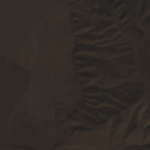
\includegraphics[width=\textwidth]{graphics/nn_visualisation/input_image_0_2.png}
        \caption{optical}
        \label{fig:nn_vis_conv_filters_inp_1}
    \end{subfigure}
    ~
    \begin{subfigure}[b]{0.25\textwidth}
        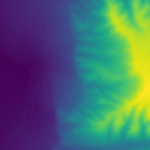
\includegraphics[width=\textwidth]{graphics/nn_visualisation/input_image_3.png}
        \caption{elevation}
        \label{fig:nn_vis_conv_filters_inp_2}
    \end{subfigure}

    \begin{subfigure}[b]{0.25\textwidth}
        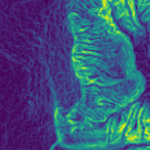
\includegraphics[width=\textwidth]{graphics/nn_visualisation/input_image_4.png}
        \caption{slope}
        \label{fig:nn_vis_conv_filters_inp_3}
    \end{subfigure}
    ~
    \begin{subfigure}[b]{0.25\textwidth}
        \includegraphics[width=\textwidth]{graphics/nn_visualisation/heatmaps_activations.png}
        \caption{Fault class activation map}
        \label{fig:nn_vis_conv_filters_cam}
    \end{subfigure}

    \caption{Sampled fault patch from the Tibet region for the convolutions visualisation}
    \label{fig:nn_vis_input}
\end{figure}

The \figurename~\ref{fig:nn_vis_input_act} presents the outputs of every filter for each convolutional layer for the
input patch. This demonstrates different features of the input patch that these filters were learnt to detect. The current
two layers detect specific features, formed by nerby pixels. Potentially, due to hierarchical nature of convolutions,
deeper convolutional layers would detect more abstract features, such as relationships between areas in different parts
of the patch.

\begin{figure}[t]
    \centering
    \begin{subfigure}[b]{\textwidth}
        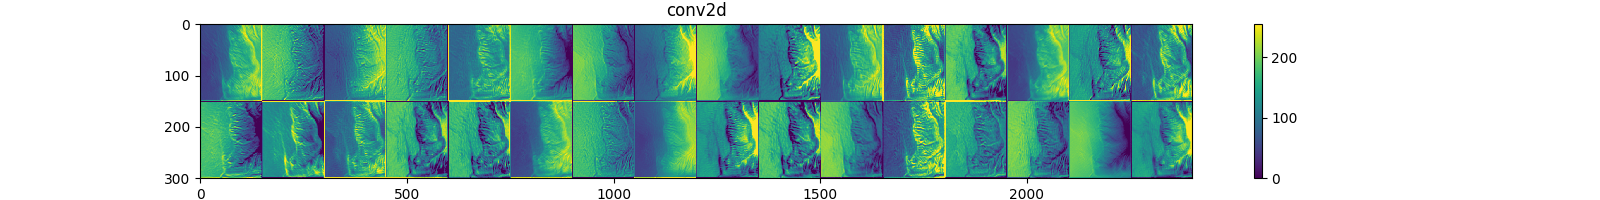
\includegraphics[width=\textwidth]{graphics/nn_visualisation/intermediate_activations_conv2d.png}
        \caption{optical}
    \end{subfigure}

    \begin{subfigure}[b]{\textwidth}
        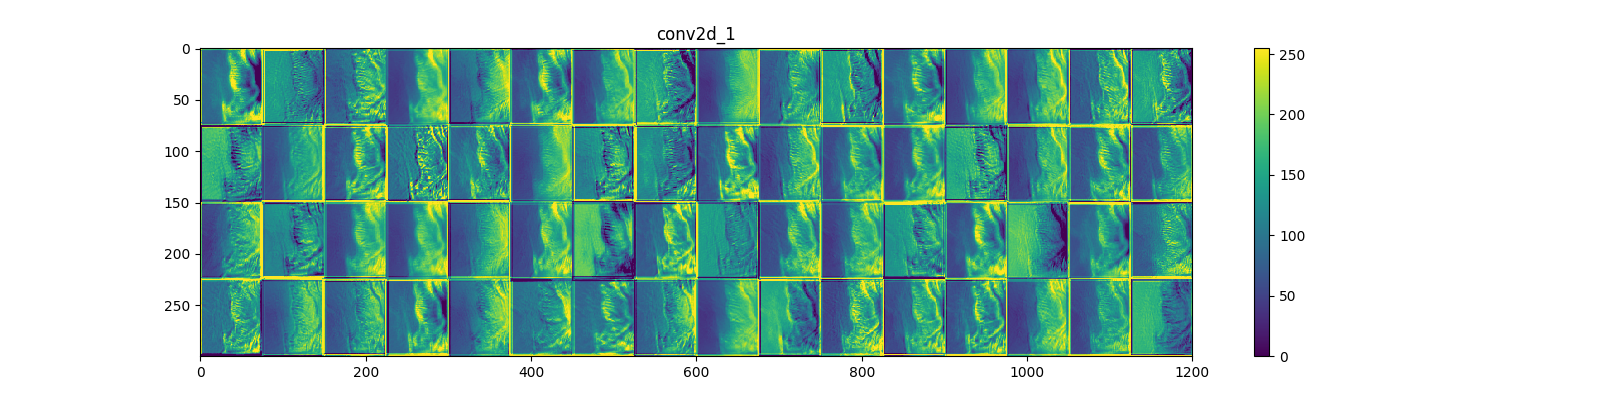
\includegraphics[width=\textwidth]{graphics/nn_visualisation/intermediate_activations_conv2d_1.png}
        \caption{elevation}
    \end{subfigure}

    \caption{Activations of convolutional layers}
    \label{fig:nn_vis_input_act}
\end{figure}

\subsection{Convolutional filters}
For this visualisation we optimise the input image to maximise the response of convolutional filters. Such
optimisations are usually used for deeper convolutions only due to the locality of patterns learn by first convolutions.
Nevertheless, we provide the results for elevation and slope channels of the input patches that maximise some of the
convolutional layers outputs in \figurename~\ref{fig:nn_vis_conv_filters}. Potentially, this demonstrates that the data
size should be increased to produce more meaningful maximising images even for the initial layers.

\begin{figure}[t]
    \centering
    \begin{subfigure}[b]{0.4\textwidth}
        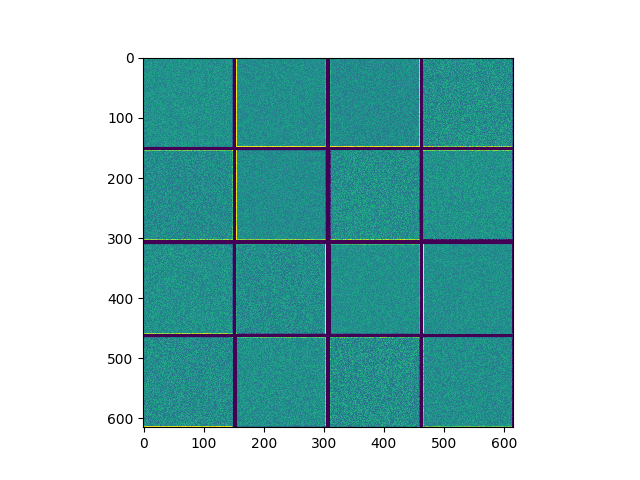
\includegraphics[width=\textwidth]{graphics/nn_visualisation/convnet_filters_elevation_conv2d.png}
        \caption{elevation, conv1}
    \end{subfigure}
    ~
    \begin{subfigure}[b]{0.4\textwidth}
        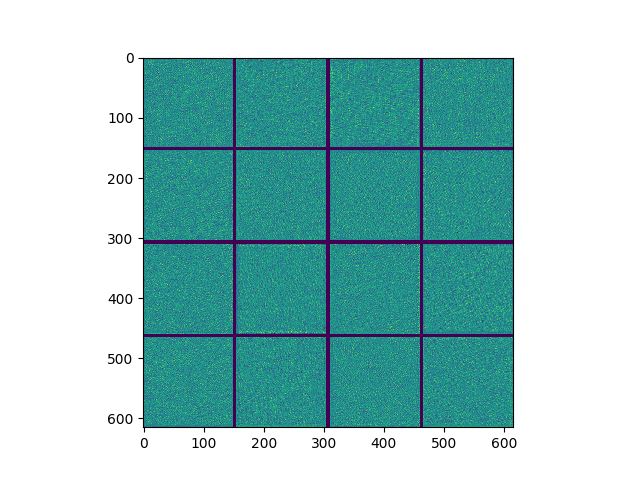
\includegraphics[width=\textwidth]{graphics/nn_visualisation/convnet_filters_elevation_conv2d_1.png}
        \caption{elevation, conv2}
    \end{subfigure}

    \begin{subfigure}[b]{0.4\textwidth}
        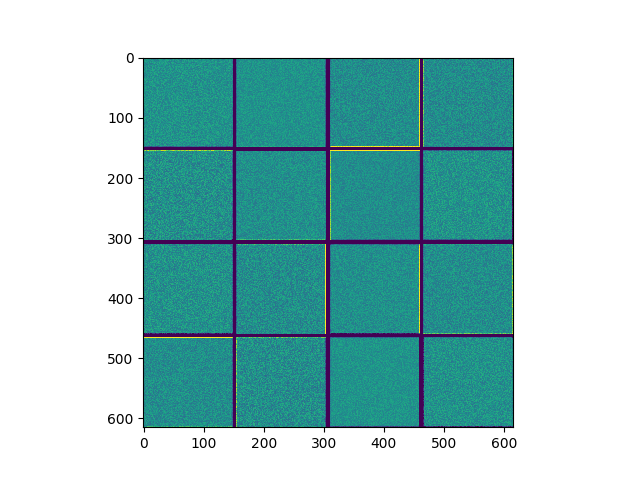
\includegraphics[width=\textwidth]{graphics/nn_visualisation/convnet_filters_slope_conv2d.png}
        \caption{slope, conv1}
    \end{subfigure}
    ~
    \begin{subfigure}[b]{0.4\textwidth}
        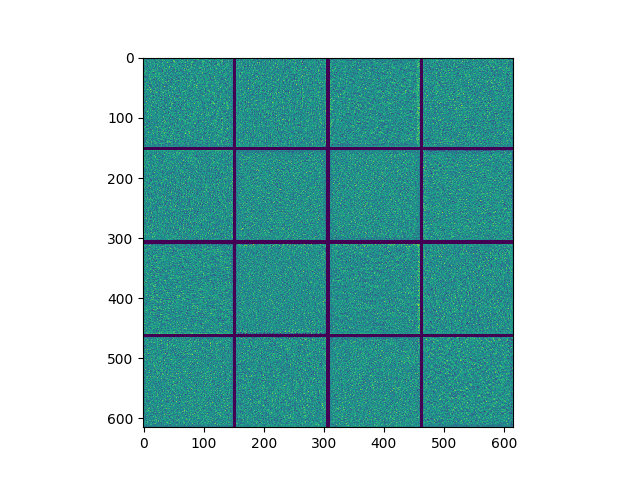
\includegraphics[width=\textwidth]{graphics/nn_visualisation/convnet_filters_slope_conv2d_1.png}
        \caption{slope, conv2}
    \end{subfigure}

    \caption{Maximisations of convolutional layers responses}
    \label{fig:nn_vis_conv_filters}
\end{figure}

\subsection{Heatmaps of class activation}
In this approach we optimise the location of the patch that lead to the final classification. We compute the gradients
of the predicted class label w.r.t. the output of the every filter at the last convolutional layer, and multiply them by
the output of the corresponding filter. Averaging the resulting values by all filters produces the heatmap presented in
\figurename~\ref{fig:nn_vis_conv_filters_cam}.

This approach can be used to determine which areas of the input patch are most meaningful for the prediction as fault
and more arguably, where the fault is located. For this specific example it can be noticed that the neural network focuses
too much on the mountain areas and too little on the actual fault area and potentially the training set should more diverse
mountain areas, so that the actual fault area would be more important for classification.

\section{Channel selection}
For this experiment we test the importance of each input channel. Though it is not widely used for deep learning that is
usually used for problems with visible spectrum only, for satellite images we have a lot of different bands form satellites
in addition to the features extracted from these channels, that are used in earth science. For interpretability of the
results it is important to choose a few of the channels that are the most important for the predictions. The usual data
science approach is to greedily add the most valuable or remove the least valuable channel. In deep learning the alternative
approach is to choose the channels that maximise the gradients of the correct predictions. We choose the first approach
and run a simple experiment with addition of one channel only. This setup does not take into account the relationships
between different channels.

Here we generate 1000 images from the Nevada training dataset, 250 images from the Nevada test dataset. We first train
the model with three optical channels only, then we train the model with four channels by adding and then removing each
remaining channel. The validation accuracy is plotted in \figurename~\ref{fig:feature_selection}. Though the validation
accuracy for two class classification is low, this scenario is considerably more difficult than previous, where the
validation data was sampled from the same images as the training data.

\begin{figure}[t]
    \centering
    \begin{subfigure}[b]{0.3\textwidth}
        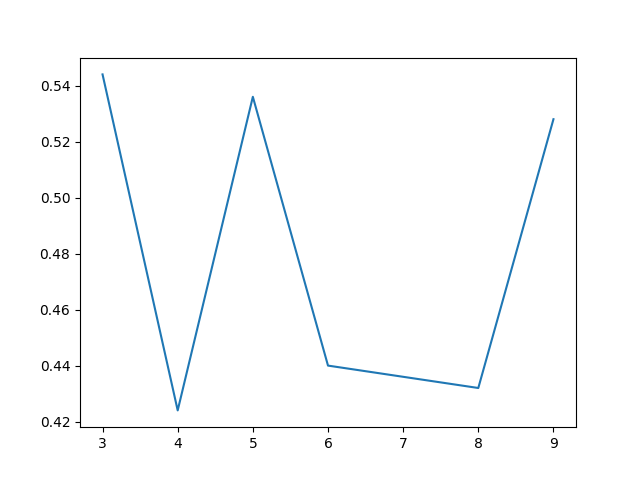
\includegraphics[width=\textwidth]{graphics/feature_selection.png}
        \caption{Features}
    \end{subfigure}

    \caption{Channel selection results. Channel numbers correspond to the sequence: elevation, slope, NIR, coastal,
    SWIR1, SWIR2, panchromatic}
    \label{fig:feature_selection}
\end{figure}

\section{Implementation}
The code is available in private repository \url{https://github.com/danilkuzin/EarthScienceFaultDetection/}
(email \texttt{danilkuzin@gmail.com} to be added). It is
implemented in python with tensorflow libraries for deep learning.

\section{Future work}
\subsection{Quality}
    \begin{itemize}
        \item Increasing the amount of data that we have may allow to increase the architecture of the network, receptive
            fields of the convolutions on later layers may provide more meaningful visualisations.
        \item There are different classes of faults mapped in the US region, such the ones in the valleys. Potentially,
            they should be separated into a different class.
        \item Predicting the physical parameters that describe the fault process.
        \item Improving the transfer learning, by training models on one area and only fine-tuning the last layer with
            the minimal data to adapt for new regions.
    \end{itemize}
\subsection{Machine learning}
    \begin{itemize}
        \item The training with lookalikes is an interesting way to use GANs by feeding faults and lookalikes and trying to
            distinguish between them.
        \item Postprocessing of predictions to get the connected lines, that can be potentially achieved with Gaussian processes,
            or denoising autoencoders.
        \item Automatically evaluate quality of mapped labels / learning from different labels for the same area (as in
            crowdsourcing with BCC)
        \item Different architecture to predict lines opposite to heatmaps. This is not well-research topic in machine learning.
    \end{itemize}
\subsection{Technical}
    \begin{itemize}
        \item Selection of the training data from the labelled image can be reassessed, for example how to sample
            uniformly from labelled lines and patches, or if it is necessary to sample from faults and lookalikes without
            intesection.
        \item Currently sampled data is stored in memory, which should be updated to loading data chunks from HDD by request.
        \item Preprocessing can include further random transformations: well-established optical transforms, such as changing
            brightness and contrast, cropping. For other channels the methods are not explored in the literature.
    \end{itemize}

\section{Conclusion}
We have demonstrated how the deep learning methods can be applied to the fault detection problem. Even with the LeNet-5
architecture we achieve the following important results:
\begin{itemize}
    \item The model trained on Tibet regions with carefully drawn training labels can be applied to the similar
    nearby regions, providing good performance.
    \item The model trained on one of the regions can be applied to the areas in a different parts of the world,
    detecting some major faults.
    \item The model trained on the publicly available fault lines without lookalikes can detect some major faults in other regions.
\end{itemize}
There are different ways to continue the research as outlined in the future work section.

\printbibliography

\section{Appendix A. Heatmaps of the predictions}
\begin{figure}[t]
    \centering
    \begin{subfigure}[b]{0.45\textwidth}
        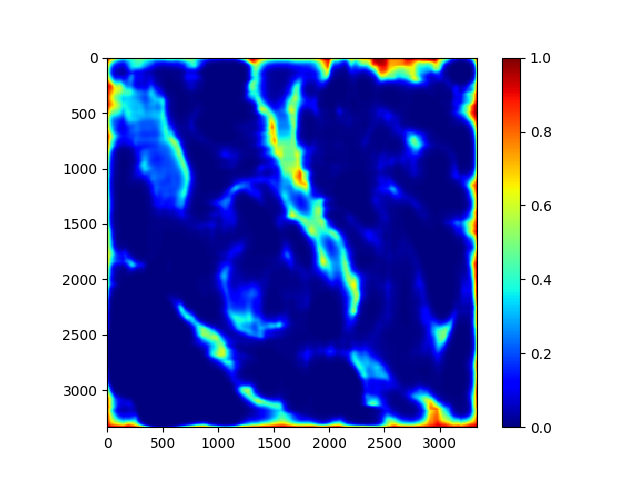
\includegraphics[width=\textwidth]{graphics/training/train_on_01_features_01234/heatmaps_faults_0.png}
        \caption{Lopukangri}
        \label{fig:heatmaps_2_Lopukangri}
    \end{subfigure}
    ~
    \begin{subfigure}[b]{0.45\textwidth}
        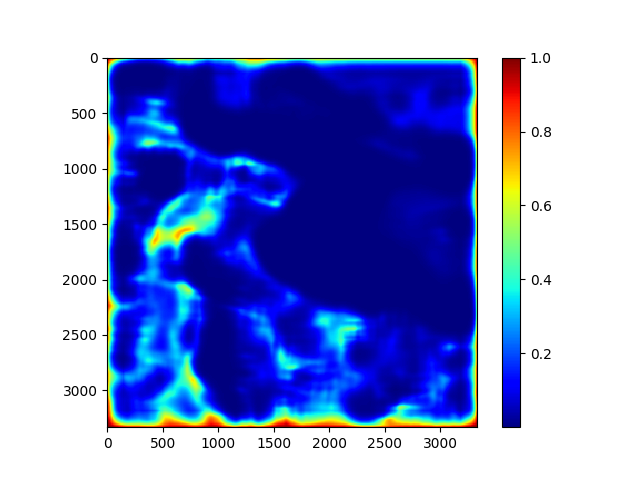
\includegraphics[width=\textwidth]{graphics/training/train_on_01_features_01234/heatmaps_faults_1.png}
        \caption{Muga Puruo}
        \label{fig:heatmaps_2_Muga_Puruo}
    \end{subfigure}

    \begin{subfigure}[b]{0.45\textwidth}
        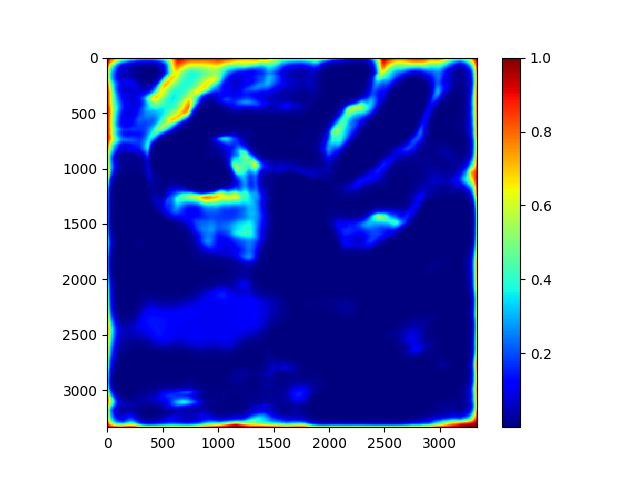
\includegraphics[width=\textwidth]{graphics/training/train_on_01_features_01234/heatmaps_faults_2.png}
        \caption{Muggarboibo}
        \label{fig:heatmaps_2_Muggarboibo}
    \end{subfigure}
    ~
    \begin{subfigure}[b]{0.45\textwidth}
        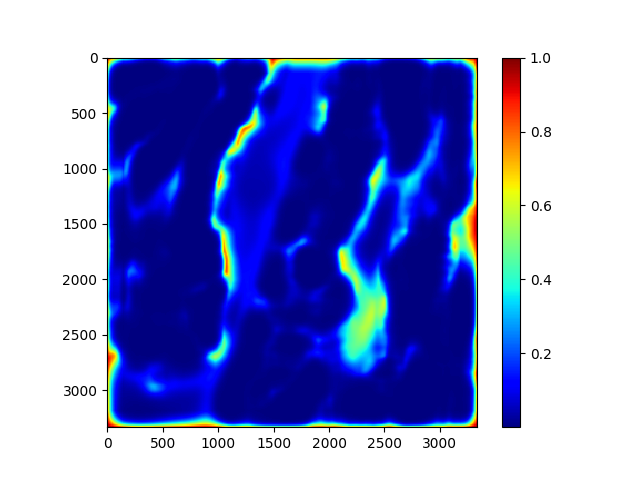
\includegraphics[width=\textwidth]{graphics/training/train_on_01_features_01234/heatmaps_faults_3.png}
        \caption{Austin-Tonopah}
        \label{fig:heatmaps_2_Austin-Tonopah}
    \end{subfigure}

    \begin{subfigure}[b]{0.45\textwidth}
        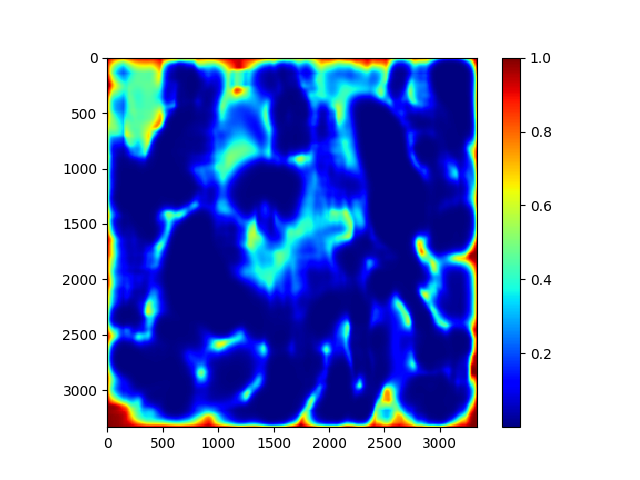
\includegraphics[width=\textwidth]{graphics/training/train_on_01_features_01234/heatmaps_faults_4.png}
        \caption{Las Vegas Nevada}
        \label{fig:heatmaps_2_Las_Vegas_Nevada}
    \end{subfigure}
    ~
    \begin{subfigure}[b]{0.45\textwidth}
        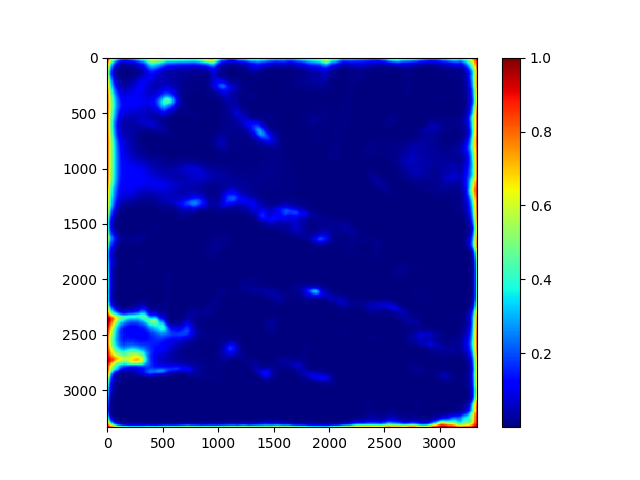
\includegraphics[width=\textwidth]{graphics/training/train_on_01_features_01234/heatmaps_faults_5.png}
        \caption{Izmir Turkey}
        \label{fig:heatmaps_2_Izmir_Turkey}
    \end{subfigure}

    \caption{Predictions based on training performed on the two Tibet regions}
    \label{fig:train_on_01_features_01234_no_additional_im}
\end{figure}

\begin{figure}[t]
    \centering
    \begin{subfigure}[b]{0.75\textwidth}
        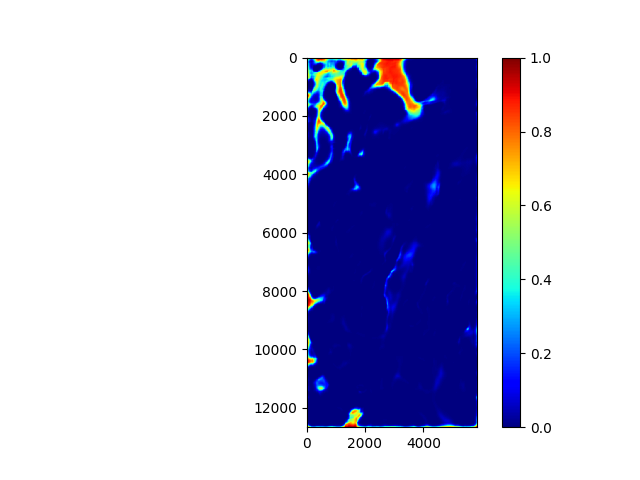
\includegraphics[width=\textwidth]{graphics/training/train_on_01_features_01234/heatmaps_faults_6.png}
        \caption{Nevada train}
    \end{subfigure}
    ~
    \begin{subfigure}[b]{0.75\textwidth}
        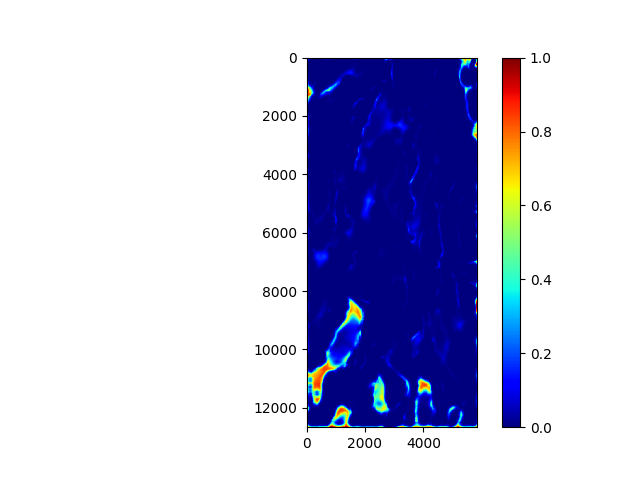
\includegraphics[width=\textwidth]{graphics/training/train_on_01_features_01234/heatmaps_faults_7.png}
        \caption{Nevada test}
    \end{subfigure}
    \caption{Predictions for US regions based on training performed on the two Tibet regions}
    \label{fig:train_on_01_features_01234_no_additional_im_us}
\end{figure}

\begin{figure}[t]
    \centering
    \begin{subfigure}[b]{0.45\textwidth}
        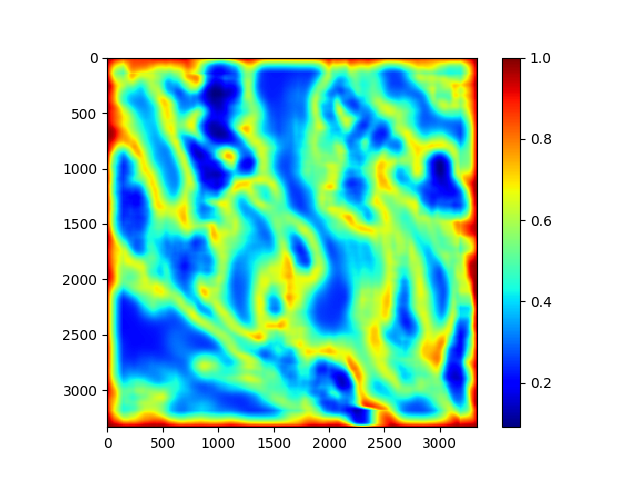
\includegraphics[width=\textwidth]{graphics/training/train_on_6_features_01234/heatmaps_faults_0.png}
        \caption{Lopukangri}
        \label{fig:heatmaps_3_Lopukangri}
    \end{subfigure}
    ~
    \begin{subfigure}[b]{0.45\textwidth}
        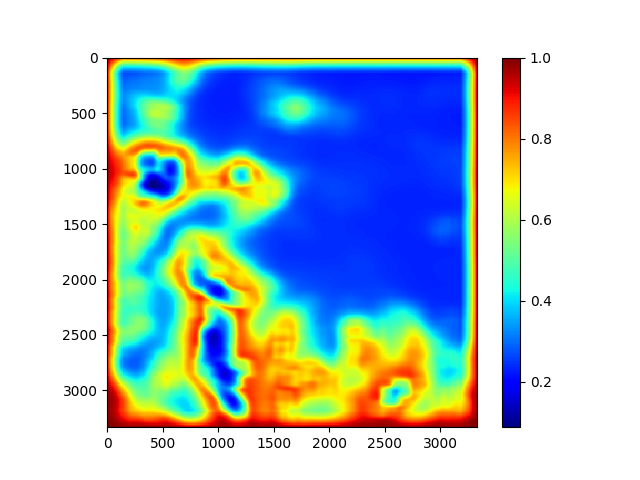
\includegraphics[width=\textwidth]{graphics/training/train_on_6_features_01234/heatmaps_faults_1.png}
        \caption{Muga Puruo}
        \label{fig:heatmaps_3_Muga_Puruo}
    \end{subfigure}

    \begin{subfigure}[b]{0.45\textwidth}
        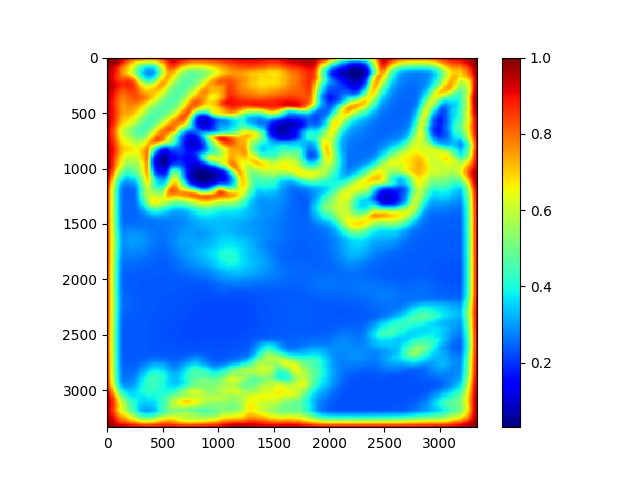
\includegraphics[width=\textwidth]{graphics/training/train_on_6_features_01234/heatmaps_faults_2.png}
        \caption{Muggarboibo}
        \label{fig:heatmaps_3_Muggarboibo}
    \end{subfigure}
    ~
    \begin{subfigure}[b]{0.45\textwidth}
        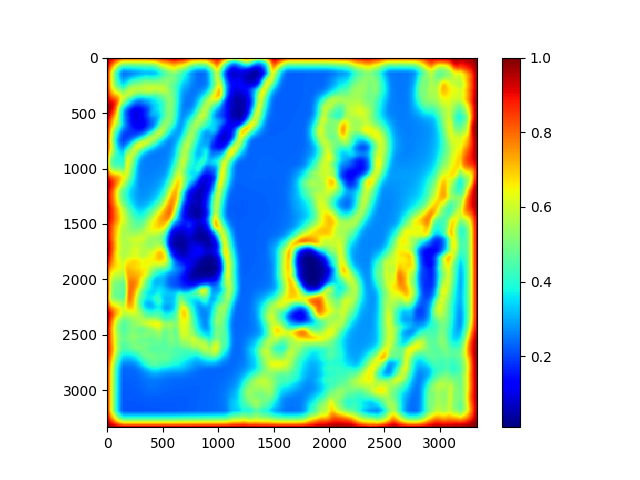
\includegraphics[width=\textwidth]{graphics/training/train_on_6_features_01234/heatmaps_faults_3.png}
        \caption{Austin-Tonopah}
        \label{fig:heatmaps_3_Austin-Tonopah}
    \end{subfigure}

    \begin{subfigure}[b]{0.45\textwidth}
        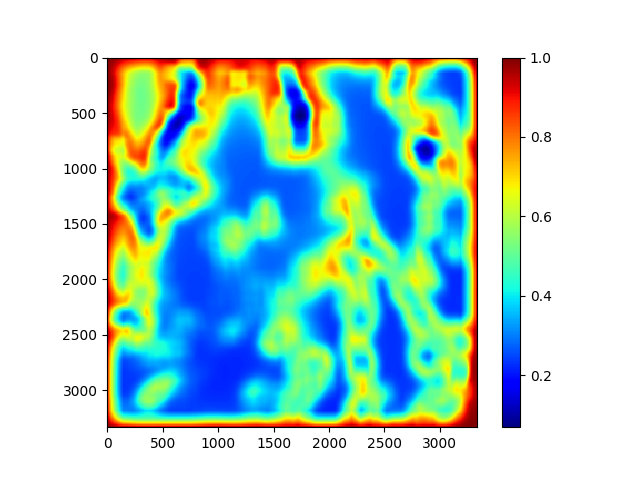
\includegraphics[width=\textwidth]{graphics/training/train_on_6_features_01234/heatmaps_faults_4.png}
        \caption{Las Vegas Nevada}
        \label{fig:heatmaps_3_Las_Vegas_Nevada}
    \end{subfigure}
    ~
    \begin{subfigure}[b]{0.45\textwidth}
        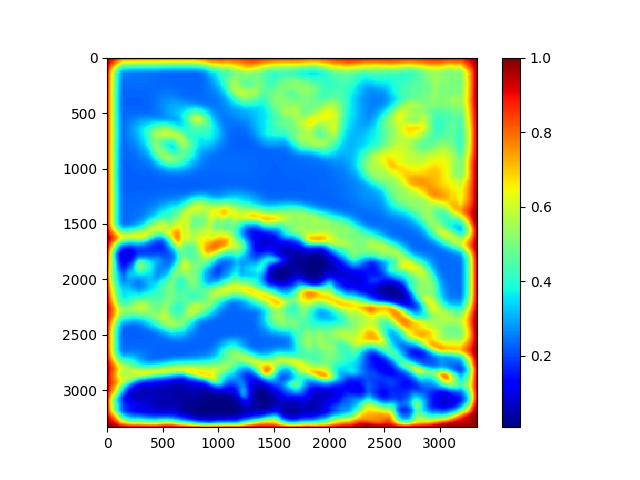
\includegraphics[width=\textwidth]{graphics/training/train_on_6_features_01234/heatmaps_faults_5.png}
        \caption{Izmir Turkey}
        \label{fig:heatmaps_3_Izmir_Turkey}
    \end{subfigure}
    \caption{Predictions based on training performed on the US Nevada train region}
    \label{fig:train_on_6_features_01234_no_additional_im}
\end{figure}

\begin{figure}[t]
    \centering
    \begin{subfigure}[b]{0.75\textwidth}
        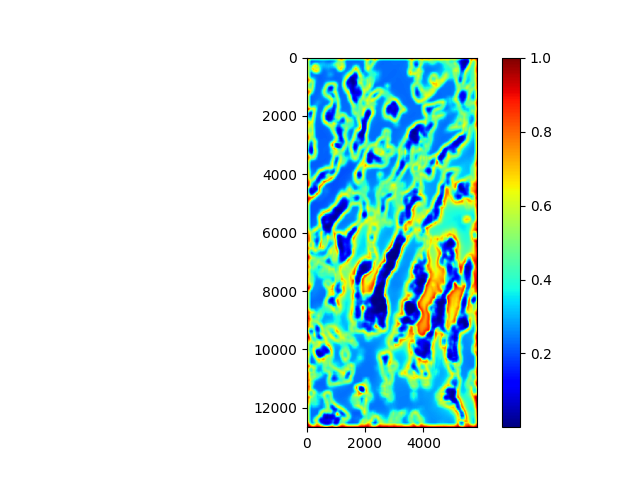
\includegraphics[width=\textwidth]{graphics/training/train_on_6_features_01234/heatmaps_faults_6.png}
        \caption{Nevada train}
    \end{subfigure}
    ~
    \begin{subfigure}[b]{0.75\textwidth}
        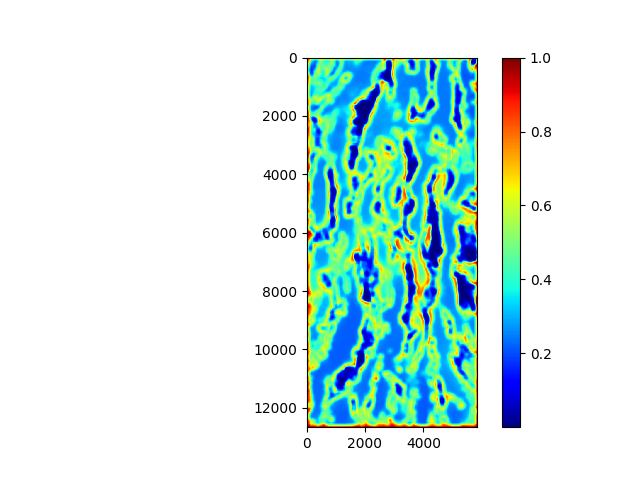
\includegraphics[width=\textwidth]{graphics/training/train_on_6_features_01234/heatmaps_faults_7.png}
        \caption{Nevada test}
    \end{subfigure}
    \caption{Predictions for US regions based on training performed on the US Nevada train region}
    \label{fig:train_on_6_features_01234_no_additional_im_us}
\end{figure}


\end{document}